\documentclass[12pt,letterpaper]{article}
\usepackage{graphicx}
\graphicspath{{images/}}
\begin{document}
\title{SSL Project Report}
\author{Kurivella Harshith\\ and\\ Nemmadi Aakash}
\date{29 april 2026}
\maketitle
\tableofcontents
\clearpage
\section{External Libraries, \\python modules and their usage in project}
\subsection{List of libraries}
\begin{itemize}
    \item \textbf{numpy} 
    \item \textbf{pygame}
    \item \textbf{matplotlib}
\end{itemize}
\subsection{List of python modules}
\begin{itemize}
    \item \textbf{sys}
    \item \textbf{time}
    \item \textbf{subprocess}
\end{itemize}
\subsection{Usage of Libraries}
\begin{description}
    \item[numpy] : -\\numpy is main core part of the project. Numpy array is used as board 
    for all the games. Its helper functions for manipulation of its arrays helps to implement 
    the game logic easily other wise would have been difficult to do. Numpy arrays slicing is 
    allows to do operations on the game board, which would be hard when done with nested loops.
    \cite{w3schools_numpy_tutorial},\cite{w3schools_numpy_reference},\cite{numpy_docs}
    \item[pygame] : -\\In this project, pygame is used to 
    visualize game from normal matrix into design game(board etc), 
    colour the board to make the game more fun; colourful,capturing the click/
    inputs from user, change upon making moves, display the winner of the game and allow user 
    to select the metric for sorting the players, various menus etc.\cite{pygame_docs}
    \item[matplotlib]: - \\matplotlib in this project is used to show the statistics of 
    players in the game hub. It is used to plot the bar graph for the top 5 players based on 
    the metric selected by user. It is also used to plot the pie chart for the distribution 
    of wins among the players.\cite{matplotlib_tutorial}   
\end{description}
\subsection{Usage of built-in python modules}
\begin{description}
    \item[sys] : -\\In this project sys is used to manipulate the arguments passed to the python 
    script i.e, game.py as command-line arguments so that the names of player can be used 
    directly.
    \item[time] : -\\The time module is used in this project to show time,date of game played by two players.
    \item[subprocess] : -\\In this project, it is used to run leaderboard.sh while running main.sh
\end{description}
\section{Features of the game hub}
\subsection{Menu}
Once users runs the bash command, A menu named "AAHa Game Hub" appears on interface.
The menu displays the all the 3 games available in the mini game hub. When the user selects a game 
the corresponding game runs.
\subsection{Games in Mini Game Hub}
The Mini game hub consists of three games: -
\begin{enumerate}
    \item TicTacToe
    \item Othello
    \item ConnectFour
\end{enumerate}
\begin{figure}[h]
    \centering
    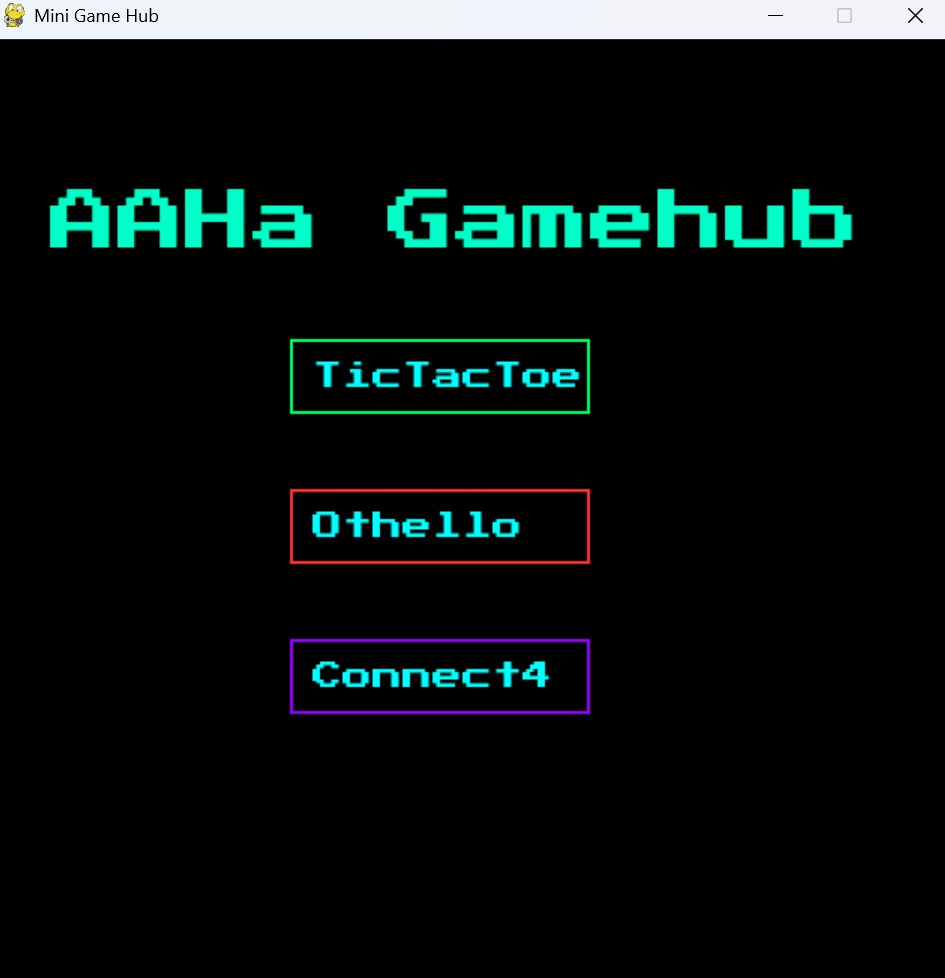
\includegraphics[width=0.80\textwidth]{Gamehub_menu}
    \caption{AAHa Game Hub menu}
    \label{fig:hame_hub_menu}
\end{figure}
\subsection{TicTacToe Game}
After the user select \emph{"TicTacToe"} game option, the game hub will lead to TicTacToe 
game interface. The board is of Bluish Grey colour. The game board is a grid of 10,10. Upon 
clicking the square box in the grid, neon blue cross appears for player 1, for the other 
player it is neon yellow colour circle. Above the game board, the interface will display 
symbol (cross for player 1 and circle for player 2) player whose turn is now. An occupied 
square will not change by either players once the square is clicked by either player. A 
player wins if consecutive 5 square boxes ( either horizontally, vertically or diagonally) 
have same symbol (neon blue cross for player 1 and neon yellow circle for player 2).There is 
quit button/option on top the game board. There is a menu option(in red colour) on top of the game board , if 
user selects the menu option, the game terminates and it goes back the main game hub menu( AAHa 
Game Hub).
\begin{figure}[h]
    \centering
    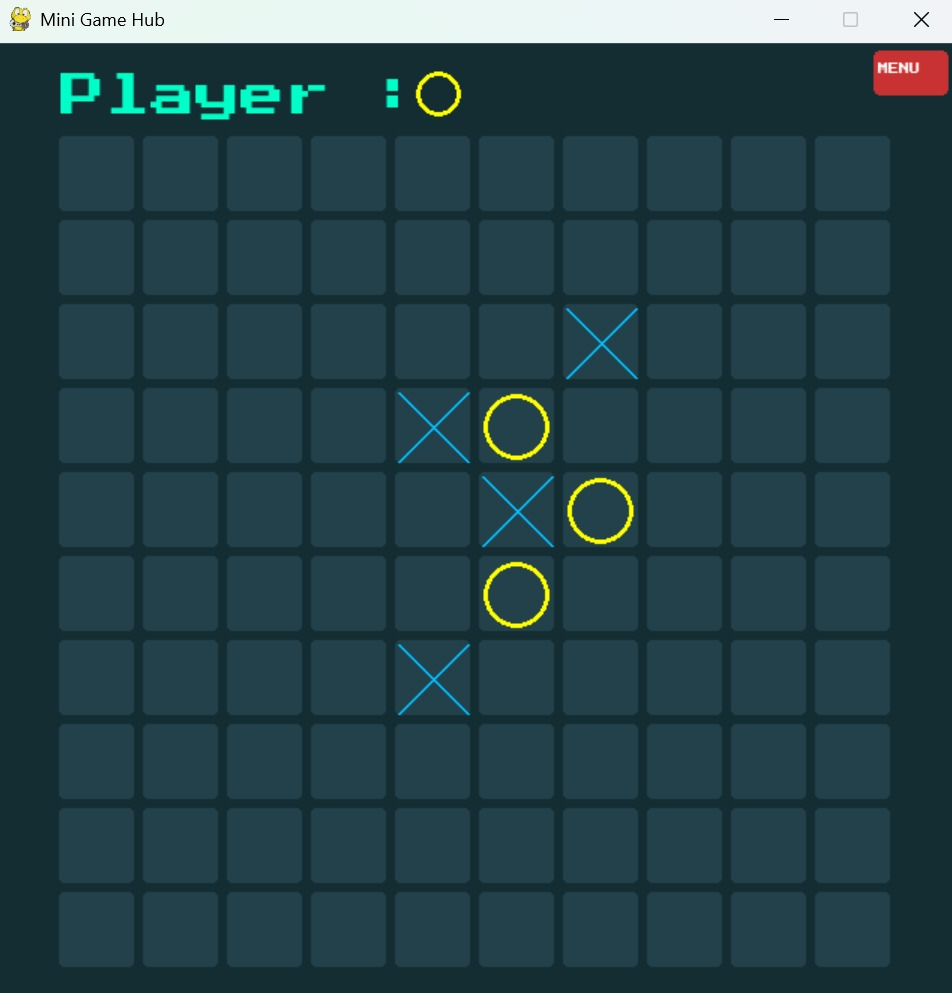
\includegraphics[width=0.50\textwidth]{TicTacToe}
    \caption{TicTacToe game}
    \label{fig:TicTacToe}
\end{figure}
\subsection{Othello(reversi) Game}
After the user select \emph{"Othello"} game option, the game hub will lead to Othello game 
interface. The board is Green. The game board is a grid of 64 discs (8,8)-standard 
Othello.Empty discs are shown in dark green circles. The game board will initially have two black 
circles and two white circles placed at 
centre of the game board with two same coloured squares arranged diagonally. Above the game 
board, the interface will show player name, current players dis'c and number of tiles each 
player's disc occupied.The interface also highlights by adding neon-blue circle to circumference of the discs  that 
are valid for current player. A player will win if he/she has \emph{more} tiles than 
opponent player when either player doesn't have valid moves left even in case where the game 
board has empty tiles in it. There is quit button/option on top the game board. There is a menu 
option(in red colour) on top of the game board , if user selects the menu option, the game terminates and it 
goes back the main game hub menu( AAHa Game Hub).
\begin{figure}[h]
    \centering
    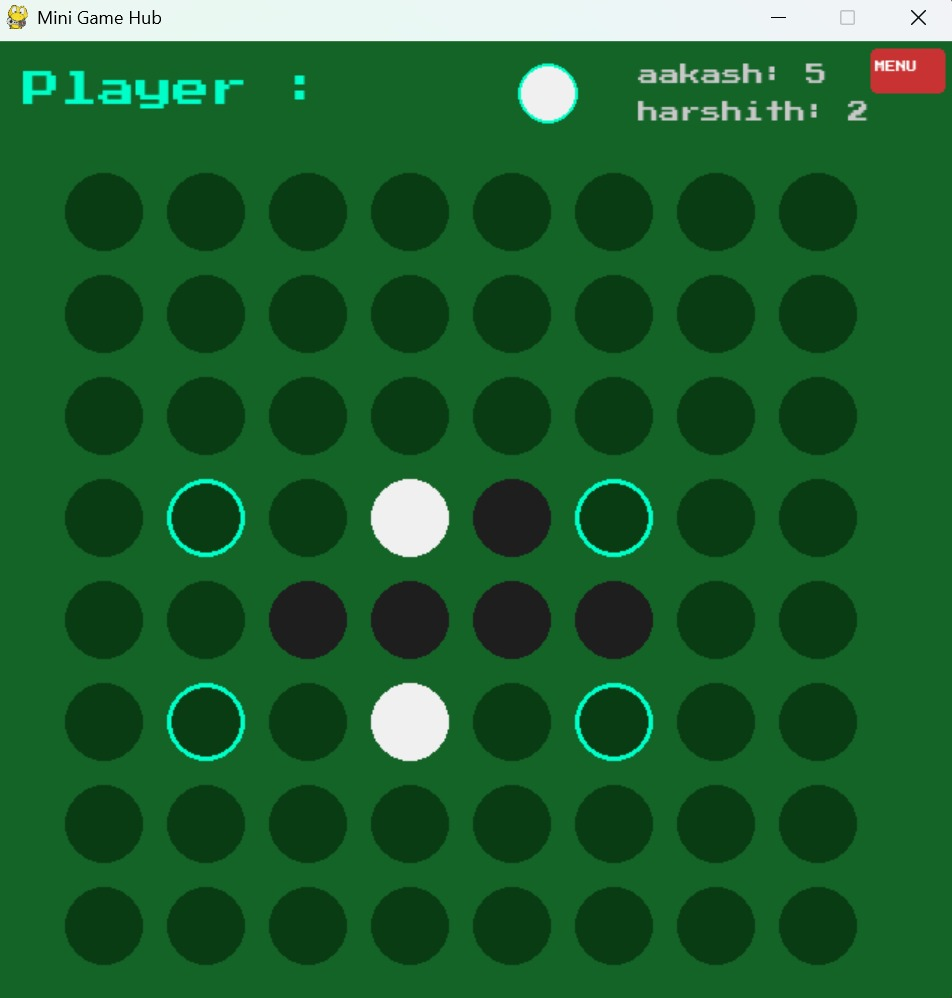
\includegraphics[width=0.50\textwidth]{Othello}
    \caption{Othello(reversi) game}
    \label{fig:Othello_reversi}
\end{figure}
\subsection{ConnectFour Game}
Once User select/clicks \emph{"Connect4"} game option, the game hub will lead to Connectfour
game interface. The game board is maroon colour consisting an array of dark maroon discs(7*7)
The game board is a grid of 49 discs(7,7). Once player clicks a incomplete column, the red 
disc occupies the lowest unoccupied position. For player 2 it is yellow colour disc. A player 
wins once the 4 consecutive discs( horizontally, vertically or diagonally) . There is quit 
button/option on top the game board. There is a menu option(in red colour) on top of the game board , if 
user selects the menu option, the game terminates and it goes back the main game hub menu
(AAHa Game Hub).
\begin{figure}[h]
    \centering
    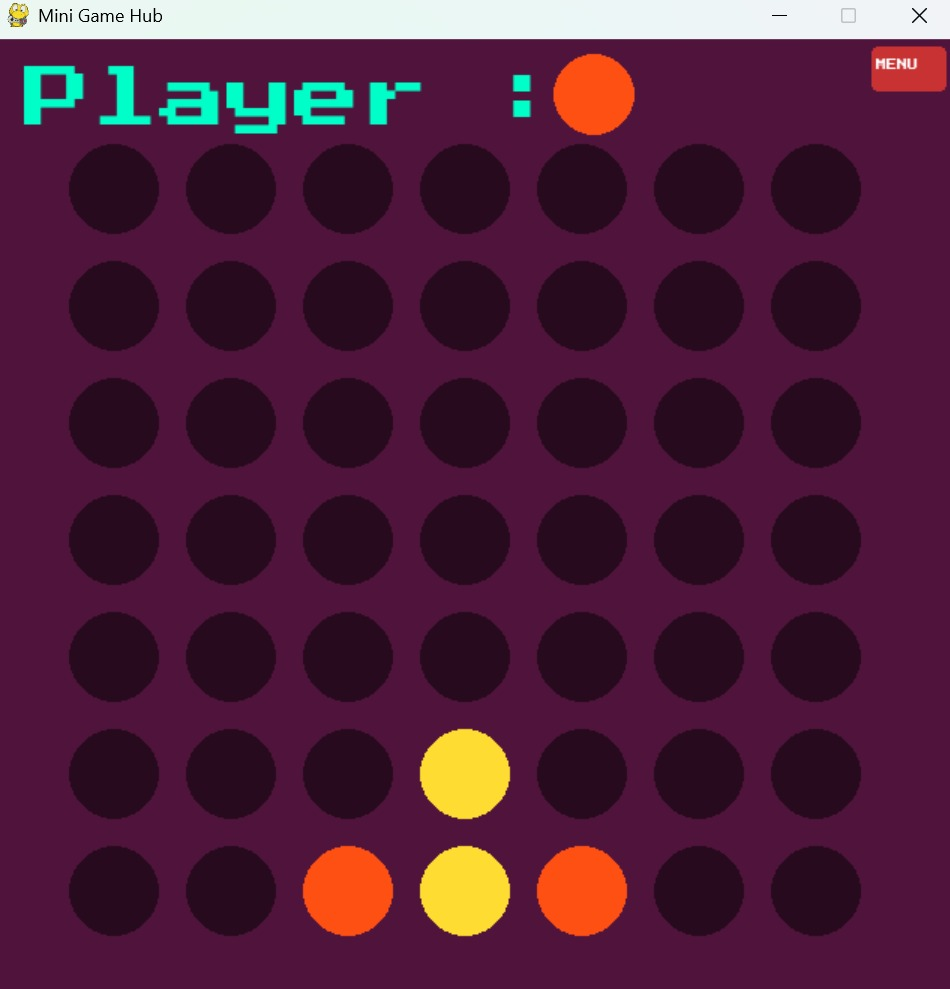
\includegraphics[width=0.50\textwidth]{Connect4}
    \caption{Connect4 game}
    \label{fig:Connect4game}
\end{figure}
\subsection{Game over menu}
After a player wins/draws the game, a menu named "Game Over" appears. It displays the winner of the game(shows draw in case of draw), shows option
\begin{enumerate}
    \item Leaderboard
    \item Statistics
    \item Restart
\end{enumerate}
\begin{figure}[h]
    \centering
    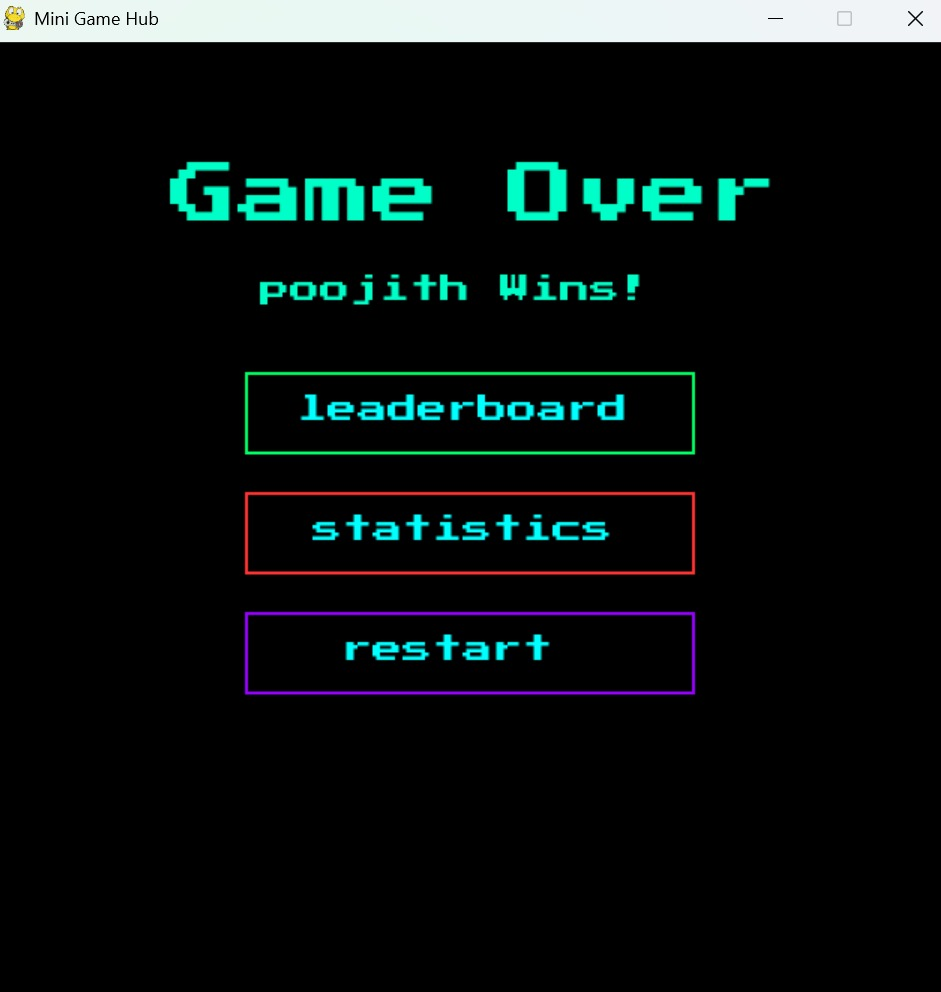
\includegraphics[width=0.50\textwidth]{Game_over_menu}
    \caption{Game over menu}
    \label{fig:Game_over}
\end{figure}
\subsection{Sort By Menu}
If user selects Leaderboard option, a menu appears named "Sort By" asking 
the metric to display all the players based on metric the user chose to sort the 
leaderboard. Sorting metrics include- 
\begin{enumerate}
    \item User/player's name
    \item Total Number of games a player played
    \item Number of games won by players
    \item Number of games lost by players
    \item Ratio of number of games won to the number of games lost
\end{enumerate}
\begin{figure}[h]
    \centering
    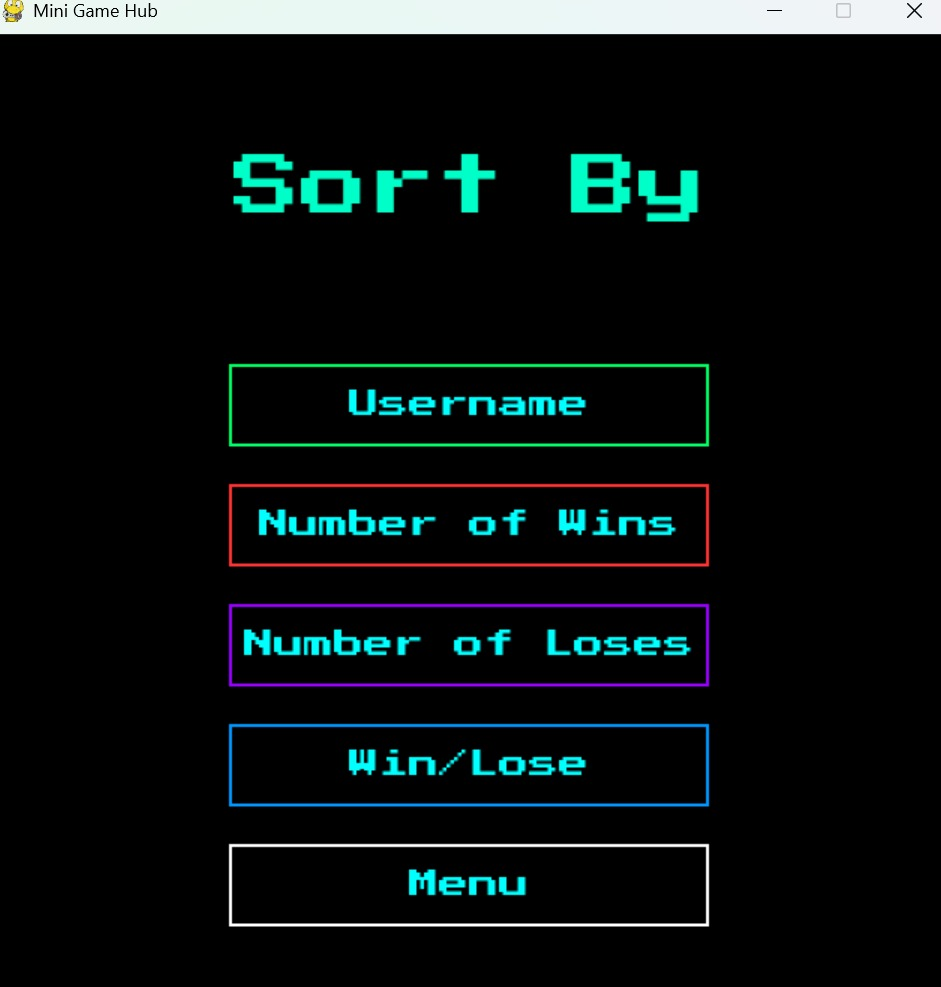
\includegraphics[width=0.50\textwidth]{Sort_by_menu}
    \caption{Sort By menu}
    \label{fig:Sort_by}
\end{figure}
Once User selects the sorting metric/criteria, A Leaderboard is printed to terminal, showing 
all players sorted based on selected criteria/metric. The leaderboard will display Player names,
their number of wins, number of losses, number of games played and ratio of number of wins 
and losses.
\subsection{Statistics}
If user selects Statistics option, the game hub will show a pi chart showing the number of times 
each game is played, two bar graphs showing - one bar graph shows the top 5 best players whereas 
the other shows top 5 worst players. Below the graphs there is menu showing an option:
Back, Menu. If user clicks/selects back option, it will come back to Game over menu.
\begin{figure}[h]
    \centering
    
\includegraphics[width=0.50\textwidth]{Statistics}
    \caption{Statistics}
    \label{fig:Statistics}
\end{figure}
\section{Code Logic and implementation }
\subsection{TicTacToe}
\subsubsection{Overview}
The Tic-Tac-Toe game is implemented using a 10×10 grid where two players take turns placing their symbols. Player 1 is represented by 'X' and Player 2 by 'O'. The objective is to align five consecutive symbols horizontally, vertically, or diagonally.
\subsubsection{Board Representation}
The game board is represented using a 2D NumPy array:
\begin{itemize}
\item Value 0 represents an empty cell
\item Value 1 represents Player 1 (X)
\item Value 2 represents Player 2 (O)
\end{itemize}
\subsubsection{Rendering the Board}
The \texttt{draw\_board()} function is responsible for:
\begin{itemize}
\item Drawing the grid using rectangles
\item Rendering X and O symbols based on board values
\item Displaying the current player indicator
\item Drawing a line across winning cells
\end{itemize}
\subsubsection{Move Handling}
The \texttt{position\_in\_table()} function:
\begin{itemize}
\item Detects mouse click events
\item Converts screen coordinates into board indices
\item Returns the selected row and column
\end{itemize}
The \texttt{make\_move()} function:
\begin{itemize}
\item Places the player's symbol if the cell is empty
\item Calls win-check logic after each move
\item Checks for draw condition if the board is full
\item Switches player turn if the game continues
\end{itemize}
\subsubsection{Win Detection Logic}
The game checks for a win using sliding window technique from NumPy:
\begin{itemize}
\item \textbf{Horizontal Check:}
A window of size 5 slides across each row. If all values match the current player, a win is declared.
\item \textbf{Vertical Check:}
A window of size 5 slides across each column to detect vertical alignment.
\item \textbf{Diagonal Check (Top-Left to Bottom-Right):}
A 5×5 sub-matrix is extracted and its main diagonal is checked.
\item \textbf{Diagonal Check (Top-Right to Bottom-Left):}
The sub-matrix is flipped and its diagonal is checked.
\end{itemize}
If any condition is satisfied:
\begin{itemize}
\item Winning cell positions are stored
\item A line is drawn across those cells
\item Game state is updated to game over
\end{itemize}
\subsubsection{Game Loop}
The \texttt{run()} function controls the main loop:
\begin{itemize}
\item Continuously updates the screen
\item Handles user input and game state
\item Stops when a player wins or the game is a draw
\end{itemize}
\subsubsection{Result Storage}
After the game ends:
\begin{itemize}
\item The result is saved into a CSV file
\item Player names, date, and game type are recorded
\end{itemize}
\subsubsection{Conclusion}
The implementation efficiently combines event handling, graphical rendering, and optimized win 
detection using NumPy. The use of sliding window technique ensures fast checking of winning 
conditions even on a larger grid.
\subsection{Othello}
\subsubsection{Overview}
The Othello game is implemented on an 8×8 grid where two players alternately place discs and 
flip opponent pieces. A move is valid only if it captures at least one opponent piece in any 
direction.
\subsubsection{Board Representation}
The board is represented using a NumPy 2D array:
\begin{itemize}
\item 0 represents an empty cell
\item 1 represents Player 1 (Black disc)
\item 2 represents Player 2 (White disc)
\end{itemize}
\subsubsection{Initial Setup}
The function \texttt{settingup\_initial\_pieces()} initializes the standard Othello starting 
configuration with four discs placed in the center of the board.

\subsubsection{Direction-Based Move Logic}
The game uses an 8-direction vector list:
[
(-1,-1), (-1,0), (-1,1), (0,-1), (0,1), (1,-1), (1,0), (1,1)
]
Each move is evaluated in all directions to determine valid flips.
\subsubsection{Valid Move and Flip Detection}
The function \texttt{\_flips\_for\_move()} performs the core logic:
\begin{itemize}
\item Checks if the selected cell is empty
\item Traverses in all 8 directions
\item Collects opponent pieces in a straight line
\item Confirms a valid move only if a player's piece encloses opponent pieces
\item Returns all pieces that must be flipped
\end{itemize}
\subsubsection{Valid Moves Generation}
The function \texttt{get\_valid\_moves()} scans the entire board and collects all positions that result in at least one valid flip for the current player.
\subsubsection{Move Execution}
The \texttt{make\_move()} function:
\begin{itemize}
\item Accepts player input (mouse click)
\item Validates move using flip detection logic
\item Places the player's disc on the board
\item Flips all opponent discs in valid directions
\item Switches player turn after a successful move
\end{itemize}
\subsubsection{Win Condition Logic}
The function \texttt{check\_win()} determines the end of the game:
\begin{itemize}
\item The game ends when no valid moves remain for both players OR the board is full
\item Player scores are calculated using NumPy sum:
\begin{itemize}
\item Player 1 score = number of cells equal to 1
\item Player 2 score = number of cells equal to 2
\end{itemize}
\item The player with the higher score is declared the winner
\end{itemize}
\subsubsection{User Interaction Handling}
The function \texttt{position\_in\_table()}:
\begin{itemize}
\item Captures mouse click events
\item Maps screen coordinates to board positions
\item Handles menu button navigation
\end{itemize}
\subsubsection{Game Loop}
The \texttt{run()} function controls the main gameplay loop:
\begin{itemize}
\item Continuously updates the board display
\item Processes player moves
\item Checks game termination conditions
\end{itemize}
\subsubsection{Result Storage}
At the end of the game:
\begin{itemize}
\item Winner and loser details are stored in a CSV file
\item Date and game type are recorded for history tracking
\end{itemize}
\subsubsection{Conclusion}
The Othello implementation uses direction-based search logic for move validation and flipping 
mechanics. The design efficiently handles game state updates, move validation, and scoring using 
NumPy operations and structured event handling.
\subsection{Connect4}
\subsubsection{Overview}
The Connect 4 game is implemented using a 7×7 grid where two players take turns dropping discs 
into columns. The objective is to connect four consecutive discs horizontally, vertically, or 
diagonally.
\subsubsection{Board Representation}
The board is represented using a 2D NumPy array:
\begin{itemize}
\item 0 represents an empty cell
\item 1 represents Player 1
\item 2 represents Player 2
\end{itemize}
\subsubsection{Rendering the Board}
The \texttt{draw\_board()} function:
\begin{itemize}
\item Draws the game background
\item Renders circular slots for each cell
\item Displays player discs based on board values
\item Shows the current player indicator
\item Displays a menu button
\end{itemize}
\subsubsection{Column Selection Logic}
The \texttt{check\_coloum()} function:
\begin{itemize}
\item Detects mouse click events
\item Checks if the click is inside any circular slot
\item Returns the column index corresponding to the clicked position
\end{itemize}
\subsubsection{Move Execution}
The \texttt{make\_move()} function:
\begin{itemize}
\item Receives the selected column
\item Iterates from bottom row upwards
\item Places the disc in the lowest available position
\item Checks for win condition after placing the disc
\item Checks for draw if the board is full
\item Switches player turn if the game continues
\end{itemize}
\subsubsection{Win Detection Logic}
Winning conditions are checked using NumPy sliding window technique:
\begin{itemize}
\item \textbf{Horizontal Check:}
A window of size 4 moves across rows to find consecutive matches.
\item \textbf{Vertical Check:}  
A window of size 4 moves across columns.
\item \textbf{Diagonal Check (Top-Left to Bottom-Right):}  
A 4×4 submatrix is extracted and its main diagonal is verified.
\item \textbf{Diagonal Check (Top-Right to Bottom-Left):}  
The submatrix is flipped and its diagonal is checked.
\end{itemize}
If any condition is satisfied:
\begin{itemize}
\item The game is marked as over
\item The current player is declared the winner
\end{itemize}
\subsubsection{Game Loop}
The \texttt{run()} function:
\begin{itemize}
\item Continuously renders the game screen
\item Handles player input
\item Executes moves until game over condition
\end{itemize}
\subsubsection{Result Handling}
After the game ends:
\begin{itemize}
\item The result is stored in a CSV file
\item Player names, date, and game type are recorded
\end{itemize}
\subsubsection{Conclusion}
The implementation uses efficient array operations and event-driven programming. The use of sliding window technique ensures fast and optimized detection of winning patterns in the grid.
\section{Hurdles, issues faced \\during the project and overcoming them}
\subsection{Hurdles}
\begin{itemize}
    \item Learning and using python took a lot of time, understanding syntax, all functions. 
    \item learning and understanding pygame without being taught in class 
    \item learning and using numpy while doing project in a very short time, trying to use numpy slicing instead nested loops
    \item Writing the games function like check\_win, make\_move etc
    \item making sure all rules of games are followed
    \item Checking the logical errors in code 
\end{itemize}
\subsection{Overcoming the hurdles}
\begin{itemize}
    \item We learnt python by referring the slides provided and python tutorial ( W3schools\cite{w3schools_python_reference}\cite{w3schools_python_tutorial} and python\cite{python_tutorial})
    \item We learnt pygame from online tutorials.\cite{pygame_docs}
    \item seeing the slides of numpy provided and numpy references, later using them and learning their syntax and usage.\cite{w3schools_numpy_tutorial}\cite{w3schools_numpy_reference}\cite{numpy_docs}
    \item From the game info \& rules, writing the functions and later adding necessary helper functions required
    \item By playing game, checking whether the game rule is obeyed or not, ensuring game flow is same as what predicted from rules.
    \item Constantly running the game, looking for errors, bugs in code by checking where rules may have been violated/disobeyed, if any rule is violated, game flow is not as expected, code is thoroughly checked for issues. 
\end{itemize}
\section{Possible project improvements \\if extra time is permitted/alloted}
if we extra time is provided/permitted we would have
\begin{itemize}
    \item Make display more creative and colourful.
    \item We would have added another game in addition to the present three games.
    \item Menus design would have been made more clean and add more necessary options
    \item Make the game code more cleaner, short and compact.
\end{itemize}
\section{References}
\bibliographystyle{plain}
\bibliography{report}
\end{document}
